The chapter will present the \acrlong{vr} system architecture, then I will talk about the hardware and software used during the development and prototyping process. I will show in detail the development process of Glimpses from Palestine application, from developing the \acrshort{vr} environment to re-building Al-Ghabisiyya in \acrlong{vr}. In the last section, I will talk about the design of the application \acrlong{ui}.

\section{Virtual Reality components}



Two main subsystems, hardware and software, make up a \acrshort{vr} system. The hardware can also be divided into \acrshort{vr} engine and I/O devices, while the software can be split into application software and database as shown in Figure \ref{fig:sys}. A \acrshort{vr} system's classic five components are Software and Database, VR Engine, I/O Devices, User and Task \citep{burdea2017virtual,Bamodu2013VirtualComponents}.

\begin{figure}[ht]
    \centering
    \includegraphics[width=0.50\textwidth]{images/VR.png}
    \caption{VR System Architecture - \citep{burdea2017virtual}}
    \label{fig:sys}
\end{figure}


\subsection{Software and Database}
Application for Virtual Reality Project is a set of tools and software to plan, develop and maintain virtual environments and the database where the information is stored. The tools can be classified as tools for modeling and development. There are many modeling tools available for \acrshort{vr} development, with 3D Max, Maya, and Creator being the most popular. Solidworks, Fusion 360, and CATIA are Engineering specific applications that could be used as well. \acrshort{vr} is a dynamic and integrative technology that borrows from many other innovations, such as real-time 3D computer graphics, tracking technology, motion synthesis, and haptic engineering, among others \citep{burdea2017virtual, Bamodu2013VirtualComponents}.

\subsection{VR Engine}
 The \acrshort{vr} engine or computer system must be selected in \acrshort{vr} systems according to the application's requirement. Some of the most important factors and time-consuming activity in a \acrshort{vr} environment is graphic interface and image creation. The selection of the \acrshort{vr} engine depends on the application area, user I/O devices immersion level, and the appropriate graphical output, as it is responsible for measuring and creating visual models, rendering objects, lighting, visualization, shading, simulation and show in real-time. The computer also manages interaction with users and serves as an interface to I/O devices. The processing power of the computer is a big factor to consider when choosing the \acrshort{vr} engine, and the processing power of the computer is the number of senses (graphic, audio, etc.) that can be rendered as pointed in a specific time frame. The \acrshort{vr} engine is expected to recalculate the virtual world roughly every 33ms and generate more than 24fps of real-time simulation, and the corresponding graphic engine should also be able to produce stereoscopic vision. The \acrshort{vr} engine could be a regular PC with more processing power and an efficient processor for graphics or decentralized computer systems linked through a high-speed communication network \citep{burdea2017virtual, Bamodu2013VirtualComponents}.


\subsection{I/O Devices}
 The input tools are the way for communicating with the virtual world by the user. They send signals about the user's action to the system to provide the user with appropriate reactions in real-time via the output devices. They can be categorized into devices for tracking, point-input devices, bio-controllers and voice devices. Often referred to as location sensors, tracking devices are used to detect the user's position, including electromagnetic, ultrasonic, optical, mechanical and gyroscopic detectors, data goggles, neural and bio or muscle controls. Types of point-input devices provide 6 \acrfull{dof} and space or force ball. Their technology is a normal mouse adaptation with extended functionality and 3D capability. Communication of voice is a common way of human interaction. Therefore, incorporating it into a \acrshort{vr} device also feels natural. To accomplish this, voice recognition or processing software may be used \citep{burdea2017virtual, Bamodu2013VirtualComponents} .

 The output devices receive feedback from the \acrshort{vr} engine and pass it on to users to stimulate the senses through the appropriate output devices. The possible senses-based classifications of output devices are graphics (visual), audio (aural), haptic (contact or force), odor and taste. The first 3 of these are often used in \acrshort{vr} environments, though odor and taste are still rare.The stereo video screen and the \acrfull{hmd}, which offers a higher level of immersion, are two potential traditional graphics choices. In the \acrshort{hmd}, the brain interprets the two separate views generated to provide a 3D perspective of the virtual world. An important medium in \acrshort{vr} is audio or sound, its value is only matched by that of video. To make the VR experience more immersive, 3D audio can be used to produce different sounds from different locations \citep{burdea2017virtual, Bamodu2013VirtualComponents}.



\subsection{User}

The users are the main reason to keep or to improve a particular \acrshort{vr} system design depending on their responses. Some users might have motion sickness during the simulation, therefore we should know what caused it, and how to avoid it. Human behavior can not be measured mathematically, it is a qualitative data, therefore its more difficult to analyze the human-machine interaction. \acrshort{vr} has many parameters, however, \acrshort{vr} human factor studies is a series of experiments aimed at determined users to perform with \acrshort{vr} technology, and it tests usability, user safety, and any related social impact related to \acrshort{vr}. 

\begin{figure}[ht]
    \centering
    \includegraphics[width=0.40\textwidth, height=250pt]{images/VRhf.png}
    \caption{VR human factors study - \citep{burdea2017virtual}}
    \label{fig:vrhf}
\end{figure}

A great advantage of data collection in \acrlong{vr} that it can be sampled during the testing, also the researcher can have a comprehensive view while the user is immersed in the simulation. Nevertheless, while designing the experimental protocol the researcher should avoid any drawbacks, for instance, to not have a repeated subject, because it will end up with the same results because data validity comes with the subject actions. Also to avoid hardware and software problems like latency which will affect the validity and reliability of the experiment. After the data is collected and analyzed, the findings will be used to refine the user interface design, enhance the software performance or add any new features to the application \citep{burdea2017virtual}. 
 
\subsection{Task}

I talked about different applications and platforms that \acrshort{vr} made an impact on it in Chapter \ref{StateoftheArt}. There are more tasks that \acrlong{vr} can enhance their performance.

For instance, Virtual reality in manufacturing. The life cycle of the manufacturing system is based on different stages, like design, personnel training, and operation, but there are multiple domains of \acrshort{vr} in manufacturing as shows in Figure \ref{fig:vrman}. 
\begin{figure}[ht]
    \centering
    \includegraphics[width=0.50\textwidth]{images/VRmanu.png}
    \caption{Domains of VR in manufacturing - \citep{burdea2017virtual}}
    \label{fig:vrman}
\end{figure}

\textbf{Virtual prototyping}: It is an obligatory stage of the development process, where the designer can validate the design, and establish manufacturing methods. Instead of drawing on a paper Virtual reality allow the designers to receive a simulation and quick feedback for the design.


\textbf{Assembly validation}: Another stage of prototyping, if the product contains multiple parts, in this stage the separate designed parts need to be tested and see they all fit together. \acrshort{vr} allows the user to test and assemble the parts. If there are flaws found in the design, it can be modified directly. 


\textbf{Ergonomic analysis}: This is made after the physical prototype is done and exist. Virtual Reality gives the users control and feels the ergonomics of the prototype in real-time. The ergonomic analysis depends on body discomfort during the testing time. With different tools, the body ergonomics of the user and the comfort of the body is being tested during the simulation in \acrshort{vr}. 

\textbf{Plant design}: New factories and large industries need to have a plan for the construction and the flow of tasks inside the facility. That's where Virtual reality can be used for simulating the tasks flow, and the user can control equipment. Designers can run high complexity tasks that cover safety, production, and many dynamic variables. Everything can be simulated by \acrshort{vr}, before anything goes into production.  

\textbf{Training maintenance}:  Training of employees takes a lot of time and effort, also it might be dangerous. Using Virtual reality in training for the assembly line, reducing the number of errors, and the training was more efficient compared to the standard training.

\textbf{Marketing}: Virtual reality also played a good role in marketing, an example for that was at many car dealerships where they had a virtual reality room, that makes the customer interact with the car within the virtual environments and adjust the car color or the seat material \citep{burdea2017virtual}.

\section{Hardware and Development Environments}

In this section, I will mention and define the equipment and tools that I used to develop the application. The software that i used to build the application. and The camera's that was used to film the cities and locations in Palestine. I used Virtual reality headsets and headphones to test the application with users.


\subsection{Headsets}

\textbf{Google Cardboard}: The virtual reality platform was released in
2014 by Google. The platform is intended as a low-cost system to
encourage interest and development in VR applications. It was
named for its fold-out cardboard viewer. The Google Cardboard
headsets are built out of simple, low-cost components -
cardboard. Google open-sourced the schematics and the
assembly instructions freely on their site, allowing people to
assemble Cardboard themselves from readily available parts \citep{Prasuethsut2014GoogleReview}.


\textbf{Google Daydream}: Google Daydream is not made out of plastic and not cardboard. It is made out of cloth, and that makes it a light virtual reality headset. Virtual reality can be activated automatically in android devices with this headset via the \acrfull{nfc} chipset installed on the door of the headset. The smartphone does not need to be in a certain position, because Daydream will automatically align the image of the mobile to the lenses. Since it is made out of cloth, it is a very comfortable headset because of the face cushion that gives a comfortable feeling, and the thick strap that holds the whole headset around the head, like ski goggles. Nevertheless the weight, it makes the user keep playing without being tired \citep{Amadeo2016DaydreamTechnica}. 


\subsection{Cameras}
\textbf{GoPro Fusion}: The footage quality can reach up to 5.2K spherical video resolution. The GoPro fusion can be controlled via a mobile application through Bluetooth or Wi-Fi. The two lenses on the two
sides are not symmetrically aligned, they are off-axis. That helps to
process the images or the footage taken from the two lenses to not
have visible stitching or overlapping in the final image. That is a
common problem in most of the VR cameras to have a big overlapping on the final image. With a 4 microphones built-in the camera, it captures full circle audio for a spatial sound experience. The data is saved on two microSD cards one for each lens, the files need to be combined to have a final 360$^{\circ}$ video \citep{Easton2018}. The camera was used in most of the project filming material, it has the best footage quality and a perfect stabilization in the videos.


\textbf{Samsung Gear 360}: The small and rounded shape of the camera is ideal for handheld shooting, although it has a socket also for a tripod. A small LCD screen helps in navigating through the camera modes. The video resolution is 4K, while the still images are somewhat soft. The smartphone app is easy to use and clear for the user also it offers a good range of viewing options. In general, is it a small and simple camera to use \citep{DigitalCamera2018}. The camera used as a backup camera during the project. The quality is acceptable for a small and very light camera.

\subsection{Development Environments}

\acrshort{vr} technology is moving forward and designers are gradually getting access to new tools and platforms \citep{Bamodu2013VirtualComponents}. Not only in computers but also smartphones and web, \acrshort{vr} technology has found its way into different environments. In this section, I will mention the software's that I used to develop and design a smartphone \acrshort{vr} application \say{Glimpses from Palestine}. 


\textbf{Unity 3D}: Unity is one of the most famous game engines, it is a  fully integrated development engine that offers out-of-the-box capabilities for immersive 3D creations. It has a direct \acrshort{vr} mode to preview the work on any \acrlong{hmd}, which can be easier and faster for designers to boost their productivity \citep{Kim2014UsingDevelopment}. Most of the \acrlong{hmd}s are supported in Unity. Unity works with C\# and JavaScript, it is easy to learn due to the huge online community. Unity can export the work to various platforms including Mac, Web, iOS, Android, and Xbox \citep{Kim2014UsingDevelopment}. Unity's robust tool collection, interactive interface and on-the-fly testing and editing feature let developers save time and effort Unity was the best and most powerful tool to be used during the project to develop the VR experience.

\textbf{Autodesk Fusion 360}: Fusion is a cloud-based 3D modeling software where all your work and files would be saved on the cloud. You can design \acrfull{cad} and \acrfull{cam} for \acrfull{cae} tasks. For my personal experience, it was easier for me to work with Fusion since it is an engineering-based software.  Fusion can animate and make videos, also render high quality images for the designs. Nevertheless, Fusion is designed for all levels of users, from beginner to modeling to experienced engineer \citep{Cline2018FusionFabrication}. 

\section{Development \& Implementation}

In this section, I will introduce the process of building the VR application \say{Glimpses from Palestine} also how I managed to re-built Al-Ghabisiyya village in Virtual Reality, and how I modeled the terrain of the geographical area as well as placing the village on the right location of the map. In the last part, I will talk about the interface and why it is different in Virtual Reality applications. 


\subsection{Glimpses from Palestine Application}

 I examined the earlier version of \acrshort{yallah!} \acrshort{vr} application prototype, and I perceived that the data was disordered and many files were missing. To make the design more adaptable and efficient, I determined to start from the beginning and building a 360$^{\circ}$ video environment. When starting a new scene in Unity, it places the camera in the middle of the environment by default. This camera will be the user’s point of view, the camera would be enclosed by a sphere that serves as the screen of the 360$^{\circ}$ videos. As the camera is in the middle of the sphere, the videos will be displayed on the sphere surface. Essentially in Unity, the video will be presented on the external face of the sphere. Because the video is playing on the opposite side, the camera does not expose it. Therefore, it was possible to turn the player into the inner side of the sphere by using a small C\# code. Then the video can be played on the interior side of the sphere and the camera will expose the 360$^{\circ}$ videos to seem like living inside a virtual reality setting.
\begin{figure}[ht]
    \centering
    \includegraphics[width=0.90\textwidth]{images/sphere.png}
    \caption{Virtual Reality Sphere in Unity }
    \label{fig:sphere}
\end{figure}


First, I wanted to design and code a display absolutely where I could later use it as a template for other scenes. Recently, I rendered the 360$^{\circ}$ videos that were captured in multiple locations in Palestine, it took lots of computer power as two videos from the two lenses were stitched and placed in a frame. I worked on the application design during the day, and leave the laptop at night rendering the videos.

I've brought the first video to Unity, which has been jamming all the time, I heard no sound and the picture was frozen. I tried to play the video and performed well with sound on a stand-alone VR video player. I took a step back and checked the rendering configuration. The video was produced in 5.2k resolution with the spatial sound of 8 audio channels. Unity can not manage video 5.2k smoothly and can't process space audio on 8 audio channels without a third-party plugin. Once I made changes to the rendering configuration, I researched the Unity community forum for video settings. I noticed that Unity had to transcode the videos, so I transcoded the videos to the VP8 codec. After that, the videos worked smoothly.

Now I have a world of Virtual Reality, I'm inside a 360 video, and I'm looking around as I'm there. Unity automatically solved the spatial sound problem, the video's audio was analyzed, and the spatial sound functionality was given due to the spatial sound recording feature in the GoPro Fusion. This means that now the audio shifts where the user is looking, some people call it \say{3D Audio}. 

Users need to switch around different locations and cities within the application so they need a selection tool or a controller to use it for the user interface. Due to the findings in the initial pre-study at \acrshort{yallah!}'s hackathon, the application has to be developed for a smartphone to make it easier for users to access and use. However, programming the application for a certain type of controller wouldn't be efficient because not all users can afford to get controllers. But \acrshort{vr} headsets are affordable e.g.(Google Cardboard) so, I decided to add a gaze feature in the application. The gaze functionality allows users to select active items or buttons only by staring at the button or the active object within the \acrshort{vr} environment.



I used the GoogleVR Unity asset to incorporate the environmental gaze functionality. The gaze feature adds a small blue circle in the middle of the vision of users. While the user looks at a button or an active object, an animated white stripe timeline will appear around the circle. It is an interactive sequence of 3 seconds. Once it is done, like a mouse-click on the target will be triggered. 

I applied a default button from Unity for testing the gaze feature. Therefore I created another scene that contains the same components but with a different video. I added a C\# code to the button to give it the functionality of transferring the user between the scenes. 

I was searching for Palestinian villages maps to reconstruct them, but unfortunately, I couldn't find anything on the internet. I've explored blogs, forums, Facebook groups, but no results have been found. Therefore, I made contact with a Palestinian expert in the demolished and depopulated villages. Upon describing the application concept to him, he remembered that there is a man used to live in Al-Ghabisiyya village has a map for the village before 1948. I initiated a connection with the man via WhatsApp, and I told him about the application and the objective of developing it. He was very open and showed interest in the project.  
He told me the map was based on an ariel photo that was taken in 1946 by the British mandate. While discussing more details via a phone call, he told me that the only structure that still stands in Al-Ghabisiyya is the mosque. By the end of the day, he sent me a picture for the map through WhatsApp, as shown in Figure \ref{fig:ghmap}. The map had numbers on the buildings, then he followed it with a list of family names and next to it the house number of each family that is shown on the map. 
\begin{figure}[ht]
    \centering
    \includegraphics[width=0.50\textwidth, angle=270]{images/ALGHABS_MAP.jpeg}
    \caption{Al-Ghabisiyya Map}
    \label{fig:ghmap}
\end{figure} 
 
I scanned the list to find the number of the mosque, and it was 38. That will be my reference point for modeling the rest of the village in 3D. Palestineremembered.com is a website for providing specific information about every Palestinian village. It helped me to find the location of Al-Ghabisiyya on Google Maps. I found the mosque on Google Maps, although the entire area now looks like a forest. I took a screenshot of the satellite map of the village area to align it with the map of the village.

The map didn't have any scale or orientation keys I didn't know what is the east from the west. I thought to try to scale it and use the mosque as a reference, and send it back to the man, to ask him for confirmation. I used Adobe Photoshop to merge the pictures to get a better understanding of how the village looked like as shown in Figure \ref{fig:wmap}.     

\begin{figure}[ht]
    \centering
    \includegraphics[width=0.50\textwidth]{images/wr_ghb.jpeg}
    \caption{The First try of Mapping Al-Ghabisiyya}
    \label{fig:wmap}
\end{figure} 

I began preparing the village ground sketch on Adobe Illustrator after getting assurance from the man that the position of the map was right. Then in Fusion 360, I can import an \acrfull{svg} image from Illustrator as a sketch and extrude it as a model so that the buildings would have the third dimension. While drawing the map on Adobe Illustrator, I noticed that the yard of the Mosque was on the map, so I pointed out that there was a major mistake in the mapping that I sent to the man.
The mosque yard is located in front of the mosque entrance to accommodate as many people as possible during prayers. The entrance should be to the south in the direction of Mecca, and the map in Figure \ref{fig:wmap} is to the west. Therefore, in Google maps, as shown in Figure \ref{fig:stline}, I took a straight line from the mosque to Mecca to confirm my vision about the map.


\begin{figure}[ht]
    \centering
    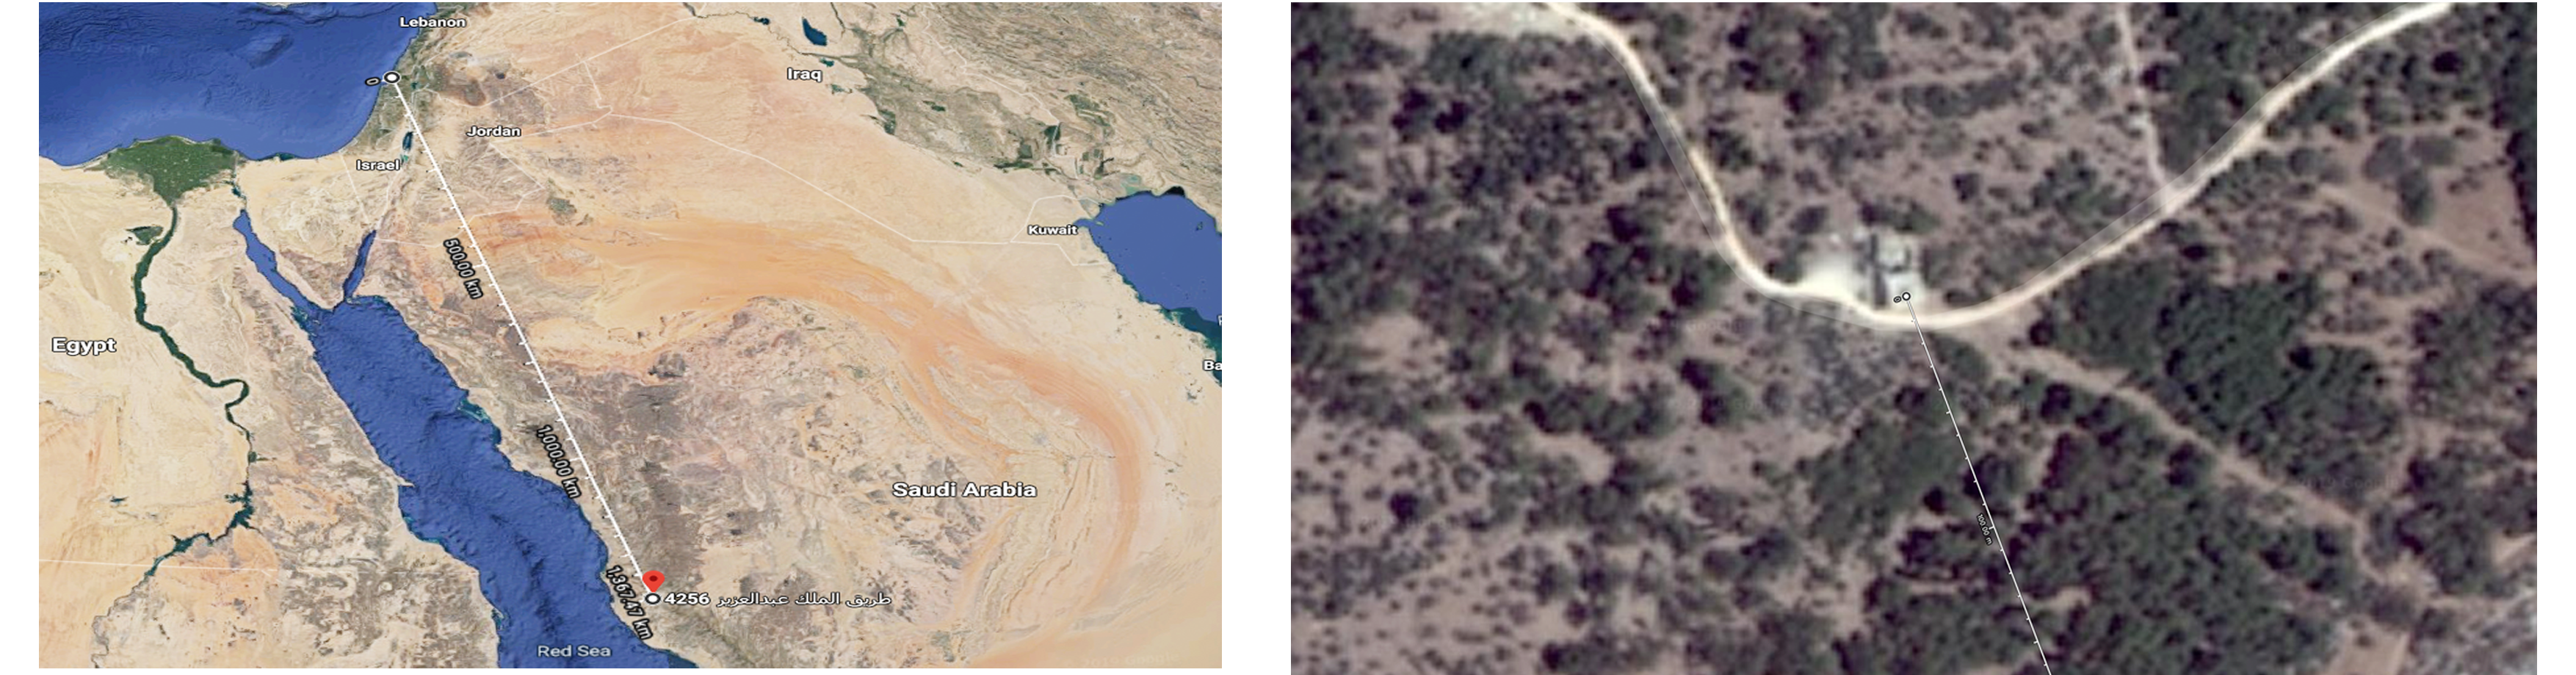
\includegraphics[width=1\textwidth]{images/stline.png}
    \caption{Al-Ghabisiyya Mosque Direction to Mecca}
    \label{fig:stline}
\end{figure} 

The location of the mosque is precisely associated with the direct line I drew, which validated the map orientation and scale without reference keys. I proceeded to scale down the map and then rotate it in the right position. Once I reached the correct orientation and map scale, the geography of the area fit exactly to the map as shown in Figure \ref{fig:scale} after all those years.


\begin{figure}[ht]
    \centering
    \includegraphics[width=0.60\textwidth]{images/scale.png}
    \caption{Al-Ghabisiyya Mapping Correction}
    \label{fig:scale}
\end{figure} 
 
After refining the map orientation, I began to build the village in 3D. It would be easier to have a high-quality map when operating on a significant detail. Unfortunately, it was a low-quality picture, but I attempted to get to most of the buildings as accurately as possible as they appeared. Furthermore, I could not get more information on building specifics, such as doors or windows. I don't just need to model the village in 3D form, but I also need to accurately determine the landscape and the location. I used 3D-map-generator.com for getting a depth map for the area as a \acrfull{png} image. I used the terrain asset in Unity and provided it with the depth map image to generate the 3D terrain model for the area around the village of Al-Ghabisiyya Figure \ref{fig:terr}.

\begin{figure}[ht]
    \centering
    \includegraphics[width=0.70\textwidth]{images/terr.png}
    \caption{Terrain}
    \label{fig:terr}
\end{figure} 


Now I have the surrounding landscape and I have the village in 3D. It is important to position the village on the terrain with the correct scaling. There's no easy way to do that except by adding the layers over each other in Photoshop using the previous method I did it with the map and the satellite image. Therefore, I took an upper terrain screenshot and applied it as a third layer on the previous work to Photoshop. I combined a satellite image, a computer-generated three-dimensional terrain and an Al-Ghabisiyya map to help me set the Al-Ghabisiyya model in the right place. Each time I shift Al-Ghabisiyya model on the terrain, I had to take a screenshot of the terrain and compare the position of the village on Photoshop, I repeated the process several times until the correct result was achieved. 
\begin{figure}[ht]
    \centering
    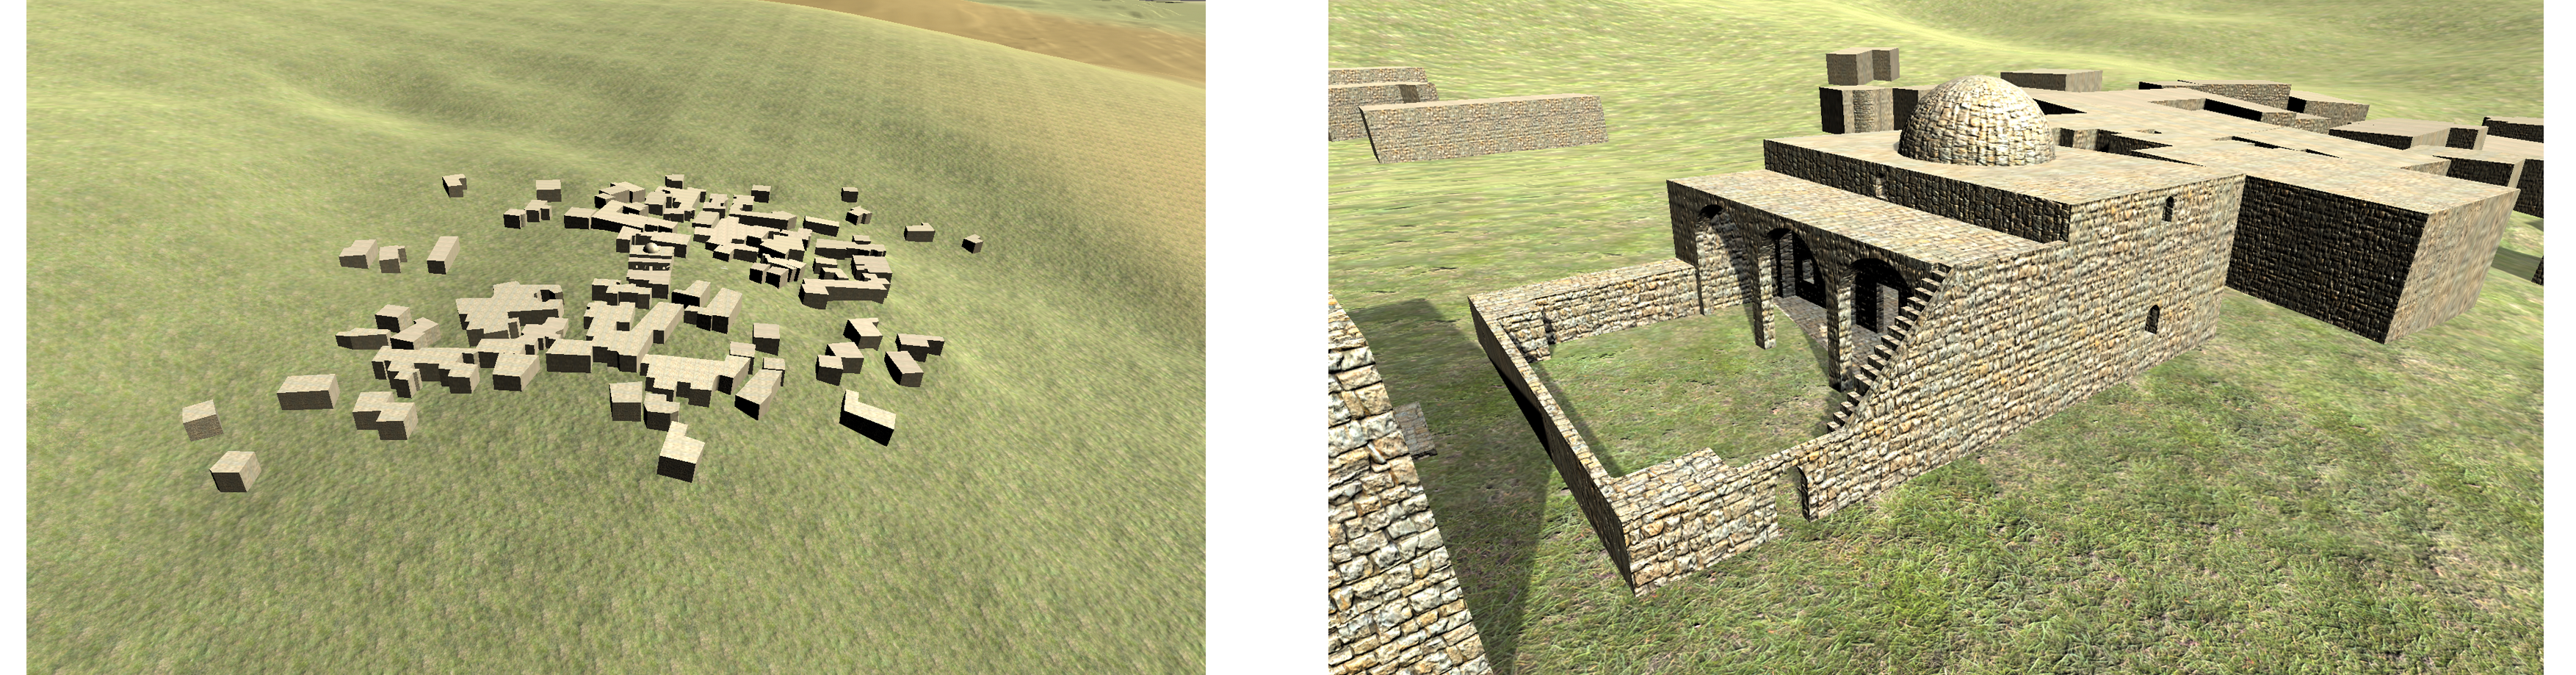
\includegraphics[width=1\textwidth]{images/Ghab_mos.png}
    \caption{3D model of Al-Ghabisiyya and the Mosque}
    \label{fig:3d}
\end{figure} 
The only building I modeled it with details was the mosque as it was the only thing that remained in Al-Ghabisiyya and I got clear pictures for it. But the rest of the buildings then I modeled them as blocks. However, as to how I saw the pictures of Al-Ghabisiyya mosque, I applied an old stone texture to the houses. Now, it is a reliable environment for the user to explore, and because I mounted cameras in various places around the village, the user can see and stand and transport between different locations in Al-Ghabisiyya.  



\subsection{User Interface}

According to \cite{burdea2017virtual} \say{In order to allow human-computer interaction it is necessary to use special interfaces designed to input a user's commands into the computer and to provide feedback from the simulation to the user} \cite [p.69]{burdea2017virtual}. 

My first attempts to create a user interface were to test the graphics in creating a reliable menu for immersive user experience. As I first needed to test the interface functionality, the appearance was a secondary task. I had a list of the cities and locations that were filmed. There were about 8 interesting scenes in each city. The first step was to create the main menu and a sub-menu, then the user could pick the location desired. The map then shows the city location with a short descriptive text on the left.  I wasn't satisfied with the concept, but I kept it just for experimentation. In a non-formal meeting with an expert on \acrshort{vr}, he noted that the buttons are not readable or easy to select. Additionally, he noted on the transition between the \acrlong{ui} and the \acrshort{vr} environment there is a white flash comes in between. He said: "This is not convenient to the users, it makes the eyes blind like a camera flash". That was a redesign catalyst for me toward the entire user experience but focused on the three pillars of \acrshort{vr}. The experience was not immersive, and the scene interactions were not designed for an environment like virtual reality. First, I removed the white flash in the transition process by changing the sphere shader from white to black. I then wanted to construct a new interface based on the principles of virtual reality. One of the most differences and problems when you design a \acrlong{ui} for \acrlong{vr} that the two-dimensional design becomes three-dimensional \citep{Kim2005GraphicalEnvironments}. 
Therefore, I decided to build a curved \acrlong{ui}, where the user can feel surrounded by it, immersed and interact with the components easier. 

\begin{figure}[ht]
    \centering
    \includegraphics[width=0.85\textwidth]{images/CurvedUI.png}
    \caption{Curved UI}
    \label{fig:CUI}
\end{figure} 


The user will be taken to the main scene of the city when the user chooses the desired city that he wants to see. Since the images are large, the selection area is by the name of the city at the bottom of the image. It's generally a well-known location in the city, in Jerusalem for example, the main scene is Damascus Gate and it is one of the main gates for Jerusalem's old city. I wanted to give information about the location for the user, it was not possible to have it during the selection process at least it wouldn't be reliable nor readable. I have implemented three virtual environment buttons that provide information about the location and a menu which allows the user to be transported to different locations or the main menu. I placed those buttons underneath the user's vision, so they do not interfere with the surrounding, but the user can see them when he looks down.  

\begin{figure}[ht]
    \centering
    \includegraphics[width=0.40\textwidth]{images/menu.png}
    \caption{VR Environment Buttons}
    \label{fig:a}
\end{figure} 

From the right a hamburger button, I made it the menu button for the user to have the ability to change the location by opening a panel and show the user multiple locations inside the city or to get back to the main menu and change the city. The panel has a transparent look with big pictures and names of other locations that the user can choose.
\begin{figure}[ht]
    \centering
    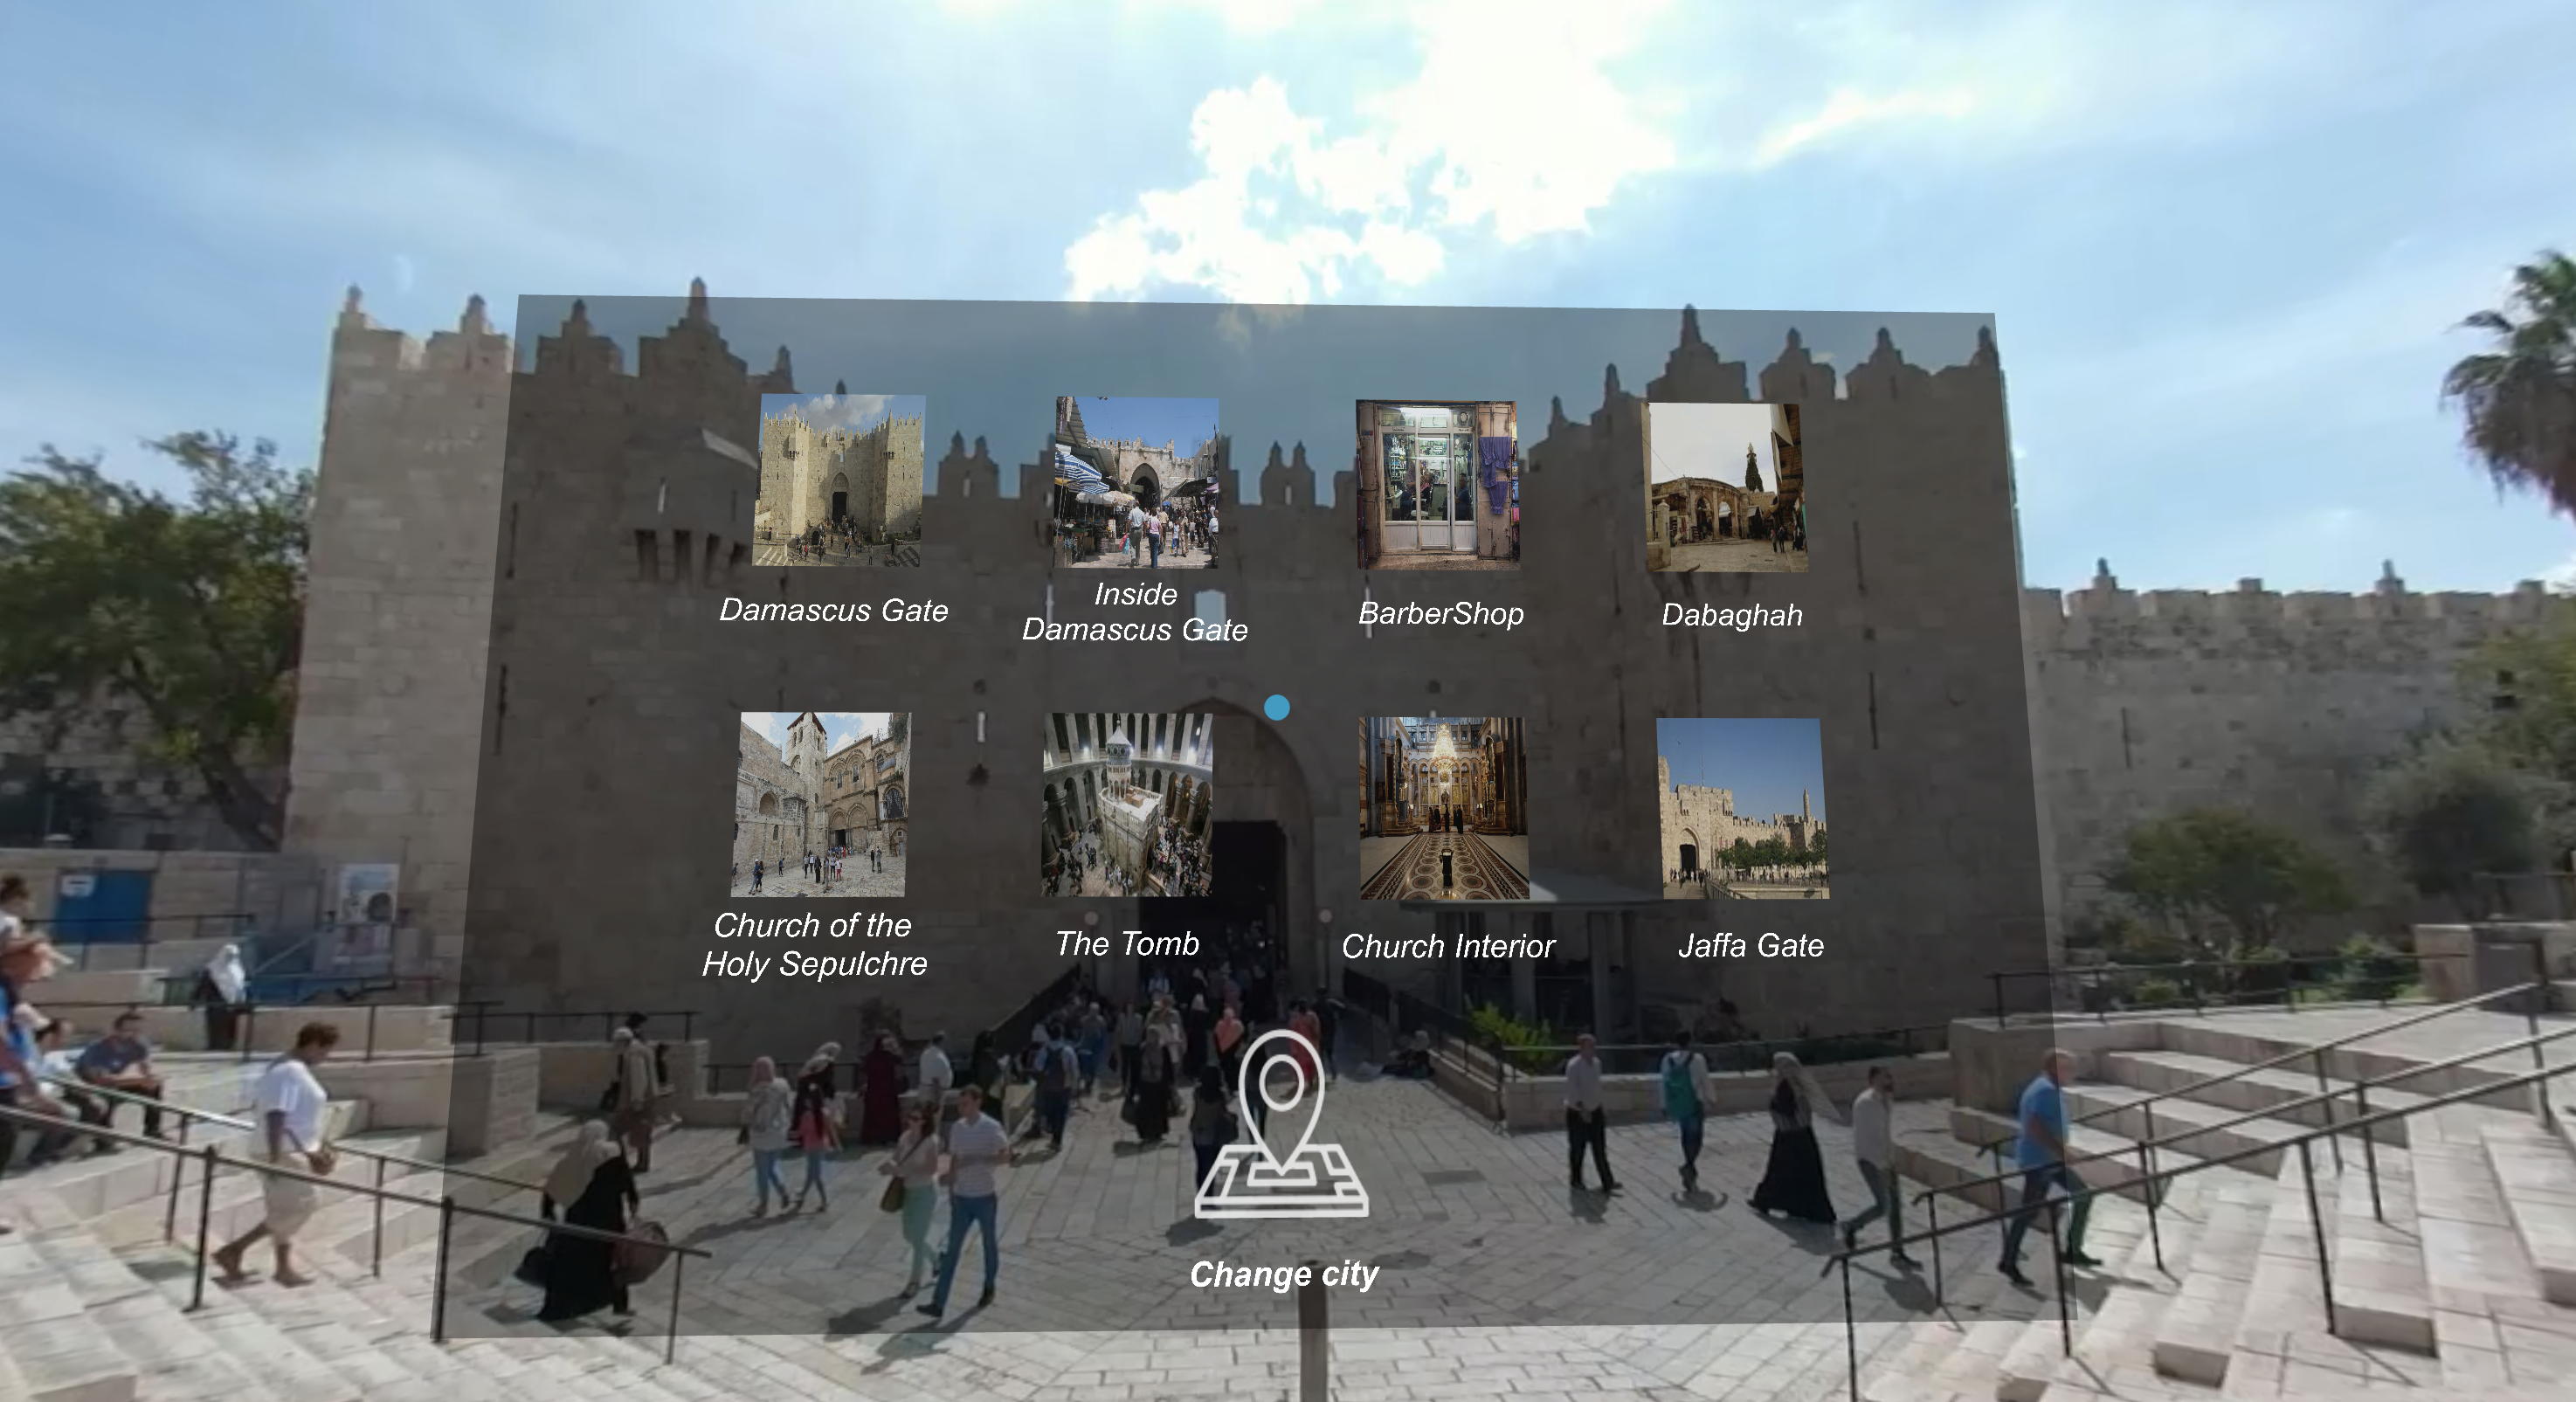
\includegraphics[width=0.60\textwidth]{images/transport.png}
    \caption{Menu Panel}
    \label{fig:mp}
\end{figure} 
The middle button is the Info button. When the user selects it, a small bar will appear at the bottom of the screen. It contains a piece of brief information about the location and a map pointing to the location.
\begin{figure}[ht]
    \centering
    \includegraphics[width=0.60\textwidth]{images/Info.png}
    \caption{Information Bar}
    \label{fig:ib}
\end{figure} 
The difference in this bar that it is moving with the user head movements. Therefore the user can look around and read the information meanwhile enjoying the location environment. 
The X button is made for closing the Menu button and also the info bar. when it is selected it will close any of the open panels. 


The user interface has been developed and tested live. I linked my mobile to Unity directly and checked the functionality of the User Interface on Google daydream. Unity sadly does not keep the modified details vibrant. Then I adjusted the layout and wrote the parameters on a paper and then put the numbers in Unity. It was an important stage in the construction of the Interface. The information bar was especially important for the best positioning. It was challenging to locate the information bar, but the live testing made it possible to find the best readable and visible location for the bar.  